\documentclass[12pt]{article}
\usepackage{url,amsmath,setspace,amssymb,amsthm,amsfonts}


\setlength{\oddsidemargin}{.25in}
\setlength{\evensidemargin}{.25in}
\setlength{\textwidth}{6.25in}
\setlength{\topmargin}{-0.4in}
\setlength{\textheight}{8.5in}

\newcommand{\heading}[5]{
   \renewcommand{\thepage}{#1-\arabic{page}}
   \noindent
   \begin{center}
   \framebox[\textwidth]{
     \begin{minipage}{0.9\textwidth} \onehalfspacing
       {\bf CS 290G -- Introduction to Modern Cryptography} \hfill #2

       {\centering \Large #5
       
       }\medskip

       {\it #3 \hfill #4}
     \end{minipage}
   }
   \end{center}
}

\newcommand{\handout}[3]{\heading{#1}{#2}{Instructor:
Stefano Tessaro}{Scribe: Shiyu Ji}{Lecture #1: #3}}

\setlength{\parindent}{0in}

\newcommand{\eqdef}{\stackrel{def}{=}}
\newcommand{\N}{\mathbb{N}}
\newcommand{\R}{\mathbb{R}}
\newcommand{\Z}{\mathbb{Z}}
\newcommand{\F}{\mathbb{F}}
\newcommand{\bits}{\{0,1\}}
\newcommand{\inr}{\in_{\mbox{\tiny R}}}
%\newcommand{\getsr}{\gets_{\mbox{\tiny R}}}
\newcommand{\getsr}{\stackrel{\$}{\gets}}
\newcommand{\st}{\mbox{ s.t. }}
\newcommand{\etal}{{\it et al }}
\newcommand{\into}{\rightarrow}

\newcommand{\Ex}{\mathbb{E}}
\newcommand{\e}{\epsilon}
\newcommand{\ee}{\varepsilon}
\newcommand{\ceil}[1]{{\lceil{#1}\rceil}}
\newcommand{\floor}[1]{{\lfloor{#1}\rfloor}}
\newcommand{\angles}[1]{\langle #1 \rangle}
\newcommand{\Com}{{\sf Com}}
\newcommand{\desc}{{\sf desc}}

\newcommand{\rightstep}[1]{%
$\underrightarrow{\quad #1 \quad}$ }

\newcommand{\leftstep}[1]{%
$\underleftarrow{\quad #1 \quad}$ }

\newcommand{\Adv}{\mathsf{Adv}}

\newcommand{\tab}{\hspace{0.3in}}
%%%%%%%%%%%%%%%%%%%%%%%%%%%%
% Theorems & Definitions


\newtheorem{theorem}{Theorem}[section]

\newtheorem{claim}[theorem]{Claim}
\newtheorem{subclaim}{Claim}[theorem]
\newtheorem{proposition}[theorem]{Proposition}
\newtheorem{lemma}[theorem]{Lemma}
\newtheorem{corollary}[theorem]{Corollary}
\newtheorem{conjecture}[theorem]{Conjecture}

\theoremstyle{definition}
\newtheorem{definition}[theorem]{Definition}
\newtheorem{construction}[theorem]{Construction}
\newtheorem{example}[theorem]{Example}
\newtheorem{algorithm1}[theorem]{Algorithm}
\newtheorem{protocol}[theorem]{Protocol}
\newtheorem{remark}[theorem]{Remark}
\newtheorem{observation}[theorem]{Observation}
\newtheorem{assumption}[theorem]{Assumption}
\newtheorem{fact}[theorem]{Fact}

%\bibliographystyle{plain}
\usepackage{tikz}
\usetikzlibrary{calc,decorations.pathreplacing}

\begin{document}
\handout{5}{Jan 21, 2016}{Pseudorandom Functions}
\section{Recap}
Last lecture we constructed a PRG with extended outputs. That is, given a PRG $G : \bits^\lambda \mapsto \bits^{\lambda+k}$, we built another generator $G_t : \bits^\lambda \mapsto \bits^{\lambda+tk}$, and we also proved that if $G$ is a PRG and $t$ is polynomial in $\lambda$, then $G_t$ is also a PRG. The proof idea is to show that for all PPT distinguisher $D$, there exists a PPT distinguisher $D^*$ s.t.
$$\Adv_{G_t,\lambda}^{prg}(D) = t\cdot \Adv_{G,\lambda}^{prg}(D^*).$$
We ``fix'' some $D$, which expects input of $\lambda+kt$ bits, and construct $D^*$ based on the fixed $D$. $D^*$ expects $\lambda+k$ bits of input.
\begin{quote}
Distinguisher $D^* (y)$: here $y\in\bits^{\lambda+k}$ (it can be $y = G(s)$, $s\getsr\bits^\lambda$ or $y\getsr\bits^{\lambda+k}$)
\begin{enumerate}
\item $i \getsr \{1,2,\cdots,t\}$.
\item {\bf run} $D_i^* (y)$ and {\bf return} its output.
\end{enumerate}
\end{quote}
Each procedure $D_i^*(y)$ runs $D$ on $(z_1,z_2,\cdots,z_t,s_t)$, where $z_1,z_2,\cdots,z_{i-1}$ are uniformly random, $(s_i, z_i)$ is given by $y$, and $z_{i+1}, \cdots, z_t, s_t$ are generated by $G$ in the following way: 
$$(s_i,z_i)\gets y,$$
$$(s_{j+1}, z_{j+1}) \gets G(s_j, z_j),$$
for all $j$ s.t. $i\leq j < t$.
At the end, $D_i^*$ outputs the output of $D$.

Our goal is to calculate the advantage $\Adv_{G,\lambda}^{prg}(D^*)$. Before that we make a few observations on the output distribution of $D_i^*$. 

Denote by $H_i(y)$ the distribution of $(z_1,z_2,\cdots,z_t,s_t)$ given to $D$ in $D_i^*(y)$.
\begin{observation}
$$\Pr [s \getsr \bits^\lambda : D_1^*(G(s))=1] = \Pr[s \getsr \bits^\lambda : D(G_t(s))=1],$$
since in $D_1^*(G(s))$ every $z_i$ is produced by $G$, i.e., $H_1(G(s))=H_0(s)$ is the distribution of $G_t(s)$ given $s\getsr\bits^\lambda$.
\end{observation}

\begin{observation}
$$\Pr [y \getsr \bits^{\lambda+k} : D_t^*(y)=1] = \Pr [(z_1, z_2, \cdots, z_t, s_t) \getsr \bits^{\lambda+tk} : D(z_1, z_2, \cdots, z_t, s_t)=1],$$
since in $D_t^*$ every $z_t$ is at uniformly random, i.e., $H_t(y) = U_{\lambda+tk}$ given $y \getsr \bits^{\lambda+k}$.
\end{observation}

\begin{observation}
For any $i\in\{1,2,\cdots,t-1\}$,
$$\Pr [y \getsr \bits^{\lambda+k} : D_i^*(y)=1] = \Pr [s \getsr \bits^\lambda : D_{i+1}^*(G(s))=1].$$
Figure \ref{fig:2h} gives the reason.
\end{observation}

\begin{figure}[!t]
\centering{}
\begin{tikzpicture}
% s_i
\node at (1.3,1) {$\cdots$};
\draw (4,0) rectangle (5,2); \node at (4.5, 1) {$s_i$};
\draw (6,0) rectangle (7,2); \node at (6.5, 1) {$s_{i+1}$};
\draw (10,0) rectangle (11,2); \node at (10.5, 1) {$s_{t-1}$};
\draw (12,0) [fill = lightgray] rectangle (13,2); \node at (12.5, 1) {$s_t$};
% z_i
\draw [fill = lightgray] (-2,2) rectangle (-1,3); \node at (-1.5, 2.5) {$z_1$}; 
\draw [fill = lightgray] (-0.5,2) rectangle (0.5,3); \node at (0, 2.5) {$z_2$};
\draw [fill = lightgray] (2,2) rectangle (3,3); \node at (2.5, 2.5) {$z_{i-1}$};
\draw [fill = lightgray] (4,2) rectangle (5,3); \node at (4.5, 2.5) {$z_i$};
\draw [fill = lightgray] (6,2) rectangle (7,3); \node at (6.5, 2.5) {$z_{i+1}$};
\draw [fill = lightgray] (10,2) rectangle (11,3); \node at (10.5, 2.5) {$z_{t-1}$};
\draw [fill = lightgray] (12,2) rectangle (13,3); \node at (12.5, 2.5) {$z_t$};
% arrows
\draw [->, thick] (5,1) -- (6,1); \node [above] at (5.5,1) {$G$};
\draw [->, thick] (7,1) -- (8,1); \node [above] at (7.5,1) {$G$};
\node at (8.5,1) {$\cdots$};
\draw [->, thick] (9,1) -- (10,1); \node [above] at (9.5,1) {$G$};
\draw [->, thick] (11,1) -- (12,1); \node [above] at (11.5,1) {$G$};
% misc
\draw [decorate,decoration={brace, amplitude=7pt}] (4,0) -- (4,2);
\node [left] at (3.8,1) {$\lambda$};
\draw [decorate,decoration={brace, amplitude=7pt}] (0.5,3) -- (0.5,2);
\node [right] at (0.7,2.5) {$k$};
\node at (-.5,1) {$H_i(U_{\lambda+k})$};
\node at (2,.3) {$(s_i,z_i)\gets y$};
\end{tikzpicture}

\vspace{.2in}

\begin{tikzpicture}
% s_i
\node at (1.3,1) {$\cdots$};
\draw (4,0) rectangle (5,2); \node at (4.5, 1) {$s$};
\draw (6,0) rectangle (7,2); \node at (6.5, 1) {$s_{i+1}$};
\draw (10,0) rectangle (11,2); \node at (10.5, 1) {$s_{t-1}$};
\draw (12,0) [fill = lightgray] rectangle (13,2); \node at (12.5, 1) {$s_t$};
% z_i
\draw [fill = lightgray] (-2,2) rectangle (-1,3); \node at (-1.5, 2.5) {$z_1$}; 
\draw [fill = lightgray] (-0.5,2) rectangle (0.5,3); \node at (0, 2.5) {$z_2$};
\draw [fill = lightgray] (2,2) rectangle (3,3); \node at (2.5, 2.5) {$z_{i-1}$};
\draw [fill = lightgray] (4,2) rectangle (5,3); \node at (4.5, 2.5) {$z_i$};
\draw [fill = lightgray] (6,2) rectangle (7,3); \node at (6.5, 2.5) {$z_{i+1}$};
\draw [fill = lightgray] (10,2) rectangle (11,3); \node at (10.5, 2.5) {$z_{t-1}$};
\draw [fill = lightgray] (12,2) rectangle (13,3); \node at (12.5, 2.5) {$z_t$};
% arrows
\draw [->, thick] (5,1) -- (6,1); \node [above] at (5.5,1) {$G$};
\draw [->, thick] (7,1) -- (8,1); \node [above] at (7.5,1) {$G$};
\node at (8.5,1) {$\cdots$};
\draw [->, thick] (9,1) -- (10,1); \node [above] at (9.5,1) {$G$};
\draw [->, thick] (11,1) -- (12,1); \node [above] at (11.5,1) {$G$};
% misc
\draw [decorate,decoration={brace, amplitude=7pt}] (4,0) -- (4,2);
\node [left] at (3.8,1) {$\lambda$};
\draw [decorate,decoration={brace, amplitude=7pt}] (0.5,3) -- (0.5,2);
\node [right] at (0.7,2.5) {$k$};
\node at (-.5,1) {$H_{i+1}(G(U_\lambda))$};
\end{tikzpicture}
\caption{The distributions $H_i(U_{\lambda+k})$ and $H_{i+1}(G(U_\lambda))$. It turns out that they are the same distribution, since $y\getsr\bits^{\lambda+k}$ and $s\getsr\bits^{\lambda}$.}
\label{fig:2h}
\end{figure}

Based on these observations, we can compute the advantage:
$$
\begin{aligned}
&\Adv_{G,\lambda}^{prg}(D^*) \\
=& \bigg| \Pr[s \getsr \bits^\lambda : D^*(G(s)) = 1] - \Pr[y \getsr \bits^{\lambda+k} : D^*(y) = 1] \bigg| \\
=& \bigg| \frac{1}{t}\sum_{i=1}^t \Pr[s \getsr \bits^\lambda : D_i^*(G(s)) = 1] - \frac{1}{t}\sum_{i=1}^t \Pr[y \getsr \bits^{\lambda+k} : D_i^*(y) = 1] \bigg| \\
=& \frac{1}{t}\bigg| \sum_{i=1}^t \Pr[s \getsr \bits^\lambda : D_i^*(G(s)) = 1] - \sum_{i=1}^t \Pr[y \getsr \bits^{\lambda+k} : D_i^*(y) = 1] \bigg| \\
=& \frac{1}{t}|p_1 - q_t| = \frac{1}{t} \Adv_{G_t, \lambda}^{prg}(D).
\end{aligned}
$$

Last lecture we also saw a concrete construction of PRG given by Blum and Micali \cite{BM84}.
Given a large prime modulus $p$, and a generator $g$ of $\Z_p^*$, the seed is $s \in \Z_p^* = \{1,2,\cdots,p-1\}$, and we build a generator $BM_t : \Z_p^* \mapsto \bits^t$ as following.
\begin{quote}
Procedure $BM_t(s)$: ($t$ is roughly larger than $\log p$)
\begin{enumerate}
\item $s_0 \gets s$.
\item {\bf for} $i=1$ to $t$ {\bf do}
\item \tab $s_i \gets g^{s_{i-1}} \mod p$.
\item \tab $z_i \gets MSB(s_i)$.
\item {\bf return} $z_1,z_2,\cdots,z_t$.
\end{enumerate}
\end{quote}
The most significant bit (MSB) is defined as:
$$MSB(x) \eqdef \begin{cases}
1, & \textrm{if } x>\frac{p-1}{2}, \\
0, & \textrm{otherwise.}
\end{cases}.$$
We can show that Blum-Micali's construction is a PRG assuming discrete logarithm problem (DLP) is hard.
\begin{theorem}
If DLP is hard to solve, then $BM_t$ is a PRG.
\end{theorem}

\section{Pseudorandom Functions}

\begin{thebibliography}{10}

\bibitem{BM84}
M. Blum and S. Micali, 1984. 
How to generate cryptographically strong sequences of pseudorandom bits. 
SIAM journal on Computing, 13(4), pp. 850-864.

\bibitem{GGM86}
O. Goldreich, S. Goldwasser. and S. Micali, 1986. 
How to construct random functions. 
Journal of the ACM (JACM), 33(4), pp.792-807.

\end{thebibliography}

\end{document}
